\documentclass{article}
\usepackage{amsmath, amsthm, amssymb}
\usepackage {mathtext}
\usepackage{amsfonts} 
\usepackage[T1,T2A]{fontenc}
\usepackage[utf8]{inputenc}
\usepackage [english, russian] {babel}
\usepackage[babel=true]{microtype}
\usepackage{caption}
\usepackage{subcaption}
\captionsetup[table]{position=t,justification=raggedleft,slc=off}
\setlength{\abovecaptionskip}{0pt}
\usepackage {geometry}
\usepackage{graphicx}
\geometry{margin=1in}
\title{Лабораторная работа №1.4.2 \\ Определение ускорения свободного падения при помощи оборотного маятника}
\author{Павел Рудачихин \\ Б04-507}
\date{4.12.2025}
\newtheorem{theorem}{Теорема}
\begin {document}
\maketitle{}
\section* {Аннотация} 

\hspace{4mm} \textbf{Цель работы:} с помощью оборотного маятника измерить величину ускорения свободного падения.

\textbf{В работе используются:} оборотный маятник, две подвесные призмы, два груза, оптоэлектронный счётчик времени и числа колебаний, подставка с остриём, консоль, линейка, штангенциркуль.

\textbf{Методы:} измерение массы с помощью весов, измерение длины с помощью линейки и штангенциркуля, измерение времени с помощью счётчика.

\section* {Теоретические сведения}

\subsection* {Физический маятник}

\hspace{4mm} \textbf{Физическим маятником} называют твёрдое тело, способное совершать 
колебания в вертикальной плоскости, будучи подвешено за одну из своих 
точек в поле тяжести. Ось, проходящая через точку подвес перпендикулярно плоскости качания, называется \textit{осью качания} маятника. 
 
При малых колебаниях период колебаний физического маятника определяется формулой 

\begin{equation}
	T = 2\pi \sqrt{\frac{I}{mgl}},
\end{equation}

где $I$ - момент инерции маятника относительно оси качания , $m$ - масса маятника , $l$ - расстояние от оси качания до центра масс маятника. Сравним эту формулу с аналогичной для периода математического маятника:

\begin{equation}
	T = 2\pi \sqrt{\frac{l_0}{g}},
\end{equation}

Введём \textit{приведённую длину} физического маятника

\begin{equation}
	l_0 := \frac{I}{ml}
\end{equation}

Математический маятник такой длины имеет тот же период колебаний, что и физический.

\begin{figure}[h!]
	\centering
	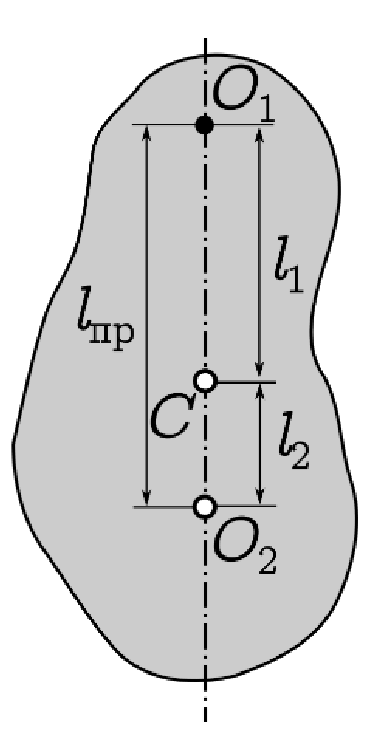
\includegraphics[width=0.2\linewidth]{1}
	\caption{Оборотный физический маятник: O и А - взаимные центры качания, С - центр масс, $l_0$ - приведённая длина.}
	\label{fig:1}
\end{figure}


Рассмотрим физический маятник с осью качания $O$ и центром масс $C$ (см. рис. 1). Отложим отрезок приведённой длины $l_0$ по прямой $OC$ и получим точку $A$. Обозначим $|OC| = l_1$, $|AC| = l_2$.

\begin{theorem}[Гюйгенса]
	 Точки $O$ и $A$ взаимны: если подвесить маятник за точку $A$, период останется прежним.
\end{theorem}

Используя теорему Гюйгенса-Штейнера, определим зависимость периода колебаний от расстояния от оси до центра масс (см. рис. 2):

\begin{equation}
	T(l_1) = 2\pi \sqrt{\frac{I_C + ml_1^2}{mgl_1}}
\end{equation}

\begin{figure}[h!]
	\centering
	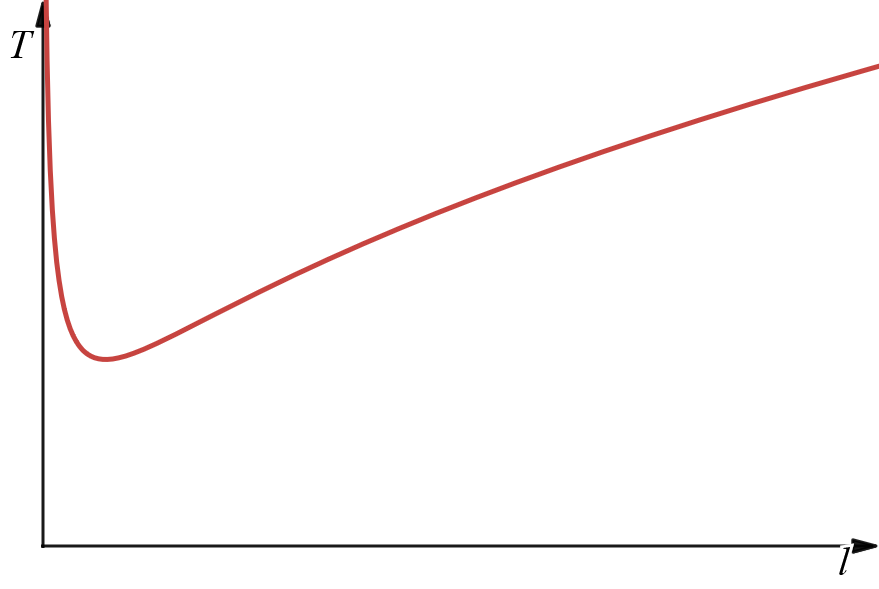
\includegraphics[width=0.7\linewidth]{2}
	\caption{График зависимости $T(l_1)$}
	\label{fig:2}
\end{figure}

Функция имеет минимум при $l_1 = \sqrt{\frac{I_C}{m}}$. В этом случае $l_1 = l_2$. 

\section* {Методика измерений}

\hspace{4mm} Пусть $L := l_1 + l_2$. При $T_1 = T_2 = T$ выполнено $L = l_0$. Выразим ускорение свободного падения из (1) и (3):

\begin{equation}
	g_0 = 4\pi^2 \frac{L}{T^2}
\end{equation} 

Однако точного совпадения периодов нельзя достичь. Поэтому определим $g$ при незначительной разнице периодов. Пусть $T := T_1$, $T + \Delta T := T_2$. Получаем:

\begin{equation}
	g = 4\pi^2 \frac{l_1^2 - l_2^2}{T_1^2 l_1 - T_2^2 l_2} = g_0 \frac{\lambda - 1}{\lambda - (1 + \tau)^2},
\end{equation} 

где $\lambda = \frac{l_1}{l_2}$, $\tau = \frac{\Delta T}{T}$. Если $\tau$ мало, то $(1+\tau)^2 \approx 1 + 2\tau$. Имеем:

\begin{equation}
	g \approx g_0 (1 + \frac{2\tau}{\lambda - 1}),
\end{equation} 

Заметим, что при $\lambda \rightarrow 1$ поправка бесконечно растёт.


\section*{Экспериментальная установка}

\begin{figure}[h!]
	\centering
	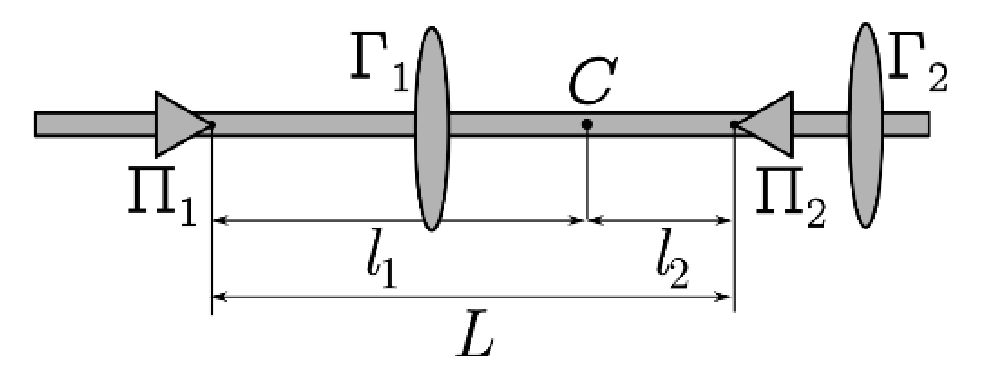
\includegraphics[width=0.7\linewidth]{3}
	\caption{Экспериментальная установка: П1 и П2 - призмы, Г1 и Г2 - грузы, С - центр масс, L - приведённая длина.}
	\label{fig:3}
\end{figure}


 \hspace{4mm}Схема установки приведена на рис. 3. 
 В работе используется маятник в форме стержня цилиндрического 
 сечения длиной около 1 м. Маятник подвешивается с помощью небольших треугольных призм (П1 и П2), острым основанием опирающихся на закреплённую на стене консоль. Ребро 
 призмы задаёт ось качания маятника. На стержне закрепляются два дополнительных груза в форме чечевицы (Г1 и Г2). 
 Фиксированное  положение  призм  однозначно  задаёт  приведённую длину маятника, а центр масс задаётся положением грузов, которое можно менять.

\section*{Используемое оборудование}

\hspace{4mm} В данной работе для измерения массы использованы цифровые \textbf{весы}. Погрешность измерения массы определена как три в последнем разряде дисплея прибора: $\Delta_{\text{m}} = \pm 0,3$ г

Погрешность \textbf{линейки} составляет $\Delta_{\text{Л}} = \pm 0,5$ мм 

Погрешность \textbf{штангенциркуля} составляет $\Delta_{\text{Ш}} = \pm 0,1$ мм 

Погрешность измерения времени на счётчике принята  $\Delta_{\text{t}} = \pm 0,01$ с

\section*{Предварительные расчёты}

\hspace{4mm} Подбор положения грузов - трудоёмкая задача, которую можно упростить благодаря предварительным расчётам по максимально упрощённой модели: маятник - тонкий однородный стержень.

Пусть $b_1$ - расстояние от груза Г1 до призмы П1, а $b_2$ - от Г2 до П2. Массы частей маятника: $m_{ст}$ - стержня, $m_{пр1}$ и  $m_{пр2}$ - подвесных призм, $m_{1}$ и $m_{2}$ - грузов. $M$ - полная масса маятника.

Пусть призмы расположены на стержне симметрично его центра масс на расстоянии $L/2$. Тогда для положения центра масс маятника относительно призмы П1 имеем:

\begin{equation}
	l_1 = \frac{1}{M} (m_{ст} L/2 + m_{пр2} L + m_{1}b_1 + m_{2}(b_2 + L))
\end{equation}

Определим все моменты инерции относительно П2.

Момент инерции стержня с призмами:

\begin{equation}
	I_{cт} = m_{ст} (\frac{l_{ст}^2}{12} + \frac{L^2}{4}) + m_{пр2}L^2
\end{equation}

Момент инерции грузов:

\begin{equation}
	I_{гр} = m_{1} (L - b_1)^2 + m_{2}b_2^2
\end{equation}

Суммарный момент по (3):

\begin{equation}
	I_{П} = MLl_2
\end{equation}

Расчёт проводится по следующему алгоритму:

\begin{enumerate}
	\item Задаём желаемое значение расстояния $l_1/l_2 = 2,5$.
	
	\item По известным массам находим $I_П$ и $I_{ст}$ 
	
	\item Варьируя длину $b_2$ в пределах от $b_2min = 0$ до $b_2max = (l - L)/2$, вычисляем по формуле (8) соответствующее положение первого груза $b_1$, а затем момент инерции грузов $I_гр$.
	
	\item Строим график $I_{гр}(b_2)$ и по точке пересечения с уровнем $I_{гр} = I_{П} - I_{ст}$ определяем искомые положения грузов (см. рис. 4)
	
	\item Проверяем, реализуемы ли расчёты на практике.
	
\end{enumerate}

\begin{figure}[h!]
	\centering
	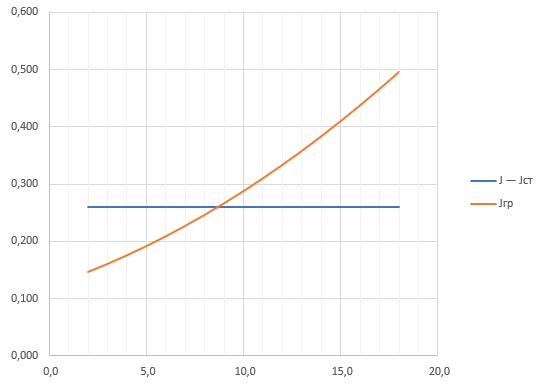
\includegraphics[width=0.7\linewidth]{5}
	\caption{График зависимости $I_{гр}(b_2)$}
	\label{fig:5}
\end{figure}


Параметры установки представлены в таблице 1. При помощи расчётной программы в ПО Microsoft Excel были получены следующие значения

\begin{equation}
	\boxed{b_1 = 20,7 \ см \ \ \ b_2 = 8,7 \ см}
\end{equation}

\begin{table}[h!]
	\centering
	\captionbox{Параметры установки}{
	\begin{tabular}{|l|r|}
		\hline
		Масса стержня $M_{ст}$, г & 1636,8 \\
		\hline
		Масса призмы $M_{пр1}$, г & 58,5 \\
		\hline
		Масса призмы $M_{пр2}$, г & 46,1 \\
		\hline
		Масса груза $M_1$, г  & 2456,0 \\
		\hline
		Масса груза $M_2$, г & 2553,8 \\
		\hline
		Длина стержня $L_{ст}$, см & 100,07 \\
		\hline
		Расстояние между призмами $L$, см & 52,07 \\
		\hline
		Отношение расстояний до центра масс $l_1/l_2$ & 2,5 \\
		\hline
	\end{tabular}}

\end{table}


\section*{Результаты измерений и наблюдений}

\hspace{4mm} Произведено по 4 измерения времени 20 колебаний при подвесе за призмы П1 и П2. Результаты приведены в таблице 2. 
\begin{table}[htbp]
	\centering
	\captionbox{Время 20 колебаний}{
	\begin{tabular}{|r|r|r|}
		\hline
		№ опыта & $t_1$, с & $t_2$, с \\
		\hline
		1        & 28,94    & 28,97 \\
		\hline
		2        & 28,94    & 28,97 \\
		\hline
		3        & 28,94    & 28,96 \\
		\hline
		4        & 28,94    & 28,96 \\
		\hline
	\end{tabular}}
\end{table}%

Определено, что случайная погрешность измерения много меньше систематической(0,003 с и 0,03 с соответственно), и отклонение $\tau = \Delta T/T \approx 0,7 $. Поэтому опыт продолжен без изменения параметров установки.

При подвесе за призму П2 время 142 колебаний составило $205,61$ с. При подвесе за призму П1 время 140 колебаний составило $202,63$ с.

Проверено влияние амплитуды на период колебаний. При вдвое меньшей амплитуде время 140 колебаний составило 202,61 c

Проверено влияние затухания колебаний. Амплитуда колебаний уменьшилась вдвое за 15 мин и 642 колебания.

\section*{Обработка результатов}

\hspace{4mm} Определим периоды колебаний на призме П1 и П2 соответственно:

\begin{equation}
	T_1 = (1,44736 \pm 0,00007) \ с \ \ \ \ T_2 = (1,44796 \pm 0,00007) \ с
\end{equation}

Имеем $\Delta T = 0,00060 \ c$ и $\tau \approx 4\cdot 10^{-4} $

\subsection*{Вычисление $g_0$}
\hspace{4mm} Определим средний период 

\begin{equation}
	T = \frac{T_1 + T_2}{2} = (1,44766 \pm 0,00007) \ с
\end{equation}

Тогда

\begin{equation}
	g_0 = 4\pi^2 \frac{L}{T^2} \approx 9,807 \ м/с^2
\end{equation}

\begin{equation}
	\varepsilon_{g_0}^2 = \varepsilon_{L}^2 + 4 \varepsilon_T^2 \ \ \ \sigma_{g_0} = \varepsilon_{g_0} g_0 \approx 0,002 \ м/с^2
\end{equation}

\subsection*{Вычисление поправки}

\begin{equation}
	(\frac{T_1}{T_2})^2 \approx 1,00083 \pm 0,00007
\end{equation}

Относительная погрешность этого отношения:

\begin{equation}
	\varepsilon = \sqrt{4 \varepsilon_{T_1}^2 + 4 \varepsilon_{T_2}^2 }
\end{equation}

\begin{equation}
	\lambda = l_1 / l_2 \approx = 2,5000 \pm 0,0007
\end{equation}

\begin{equation}
	\varepsilon_{\lambda} = \sqrt{\varepsilon_{l_1}^2 + \varepsilon_{ l_2}^2}
\end{equation}

Имеем поправку $1,0006 \pm 0,0007$

\subsection*{Окончательный результат}

\begin{equation}
	\boxed{g = 9,813 \pm 0,007 \ м/с^2}
\end{equation}

\subsection*{Оценка приближений опыта}

Период при вдвое меньшей амплитуде при подвесе за П1 составил 1,44724 с, что согласуется с периодом при обычной амплитуде в пределах погрешности.

Декремент затухания найдём по формуле

\begin{equation}
	\delta = \frac{1}{N} \ln 2 \approx 1,08 \cdot 10^{-3}
\end{equation}

Поправка к периоду

\begin{equation}
	(\frac{\delta}{2\pi})^2 \approx 2,95 \cdot 10^{-8}
\end{equation}

мала по сравнению с погрешностью.

\section*{Заключение}

\hspace{4mm} Цель работы достигнута: измерено ускорение свободного падения. 

Полученное значение ускорения свободного падения пересекается с таковым справочным для широты Москвы $9,8155 \ м/с^2$ 

Основной вклад в погрешность результата даёт нахождение
центра масс.

Все приближения опыта верны: влияние амплитуды и затуханий не превышает погрешности измерений.  

\end {document}